\subsection{Computational Fracture Mechanics}

The stress intensity factors used in this research were simulated using finite element analysis (FEA) using FRANC3D and Abaqus software \cite{f3d, Abaqus}. Abaqus served as the primary tool for creating the geometry, initial mesh discretization, application of BCs, and solution. FRANC3D was employed for tasks related to crack insertion and SIF computation. Abaqus' Python interface was used to generate the model geometries.

A local-global sub-modeling approach was employed within FRANC3D which involved dividing the geometry into two components: the global model, which encompassed the boundary conditions, and the local model, containing the region where the crack would be inserted. The local model is used in FRANC3D, where the crack is inserted using a crack front template consisting of rings of hexagonal elements, with an inner ring of quarter-point elements surrounding the crack front, allowing for SIF computations Fig. \ref{fig:f3d_mesh}. After crack insertion the local model was re-meshed, preserving the nodal locations on the cut faces (i.e. local-global boundary) for later coherency with the global model. The complete model, with the inserted crack, was subsequently solved using Abaqus. This process is illustrated in Fig. \ref{fig:f3d_abq_flow}.



\begin{figure}
  \centering
  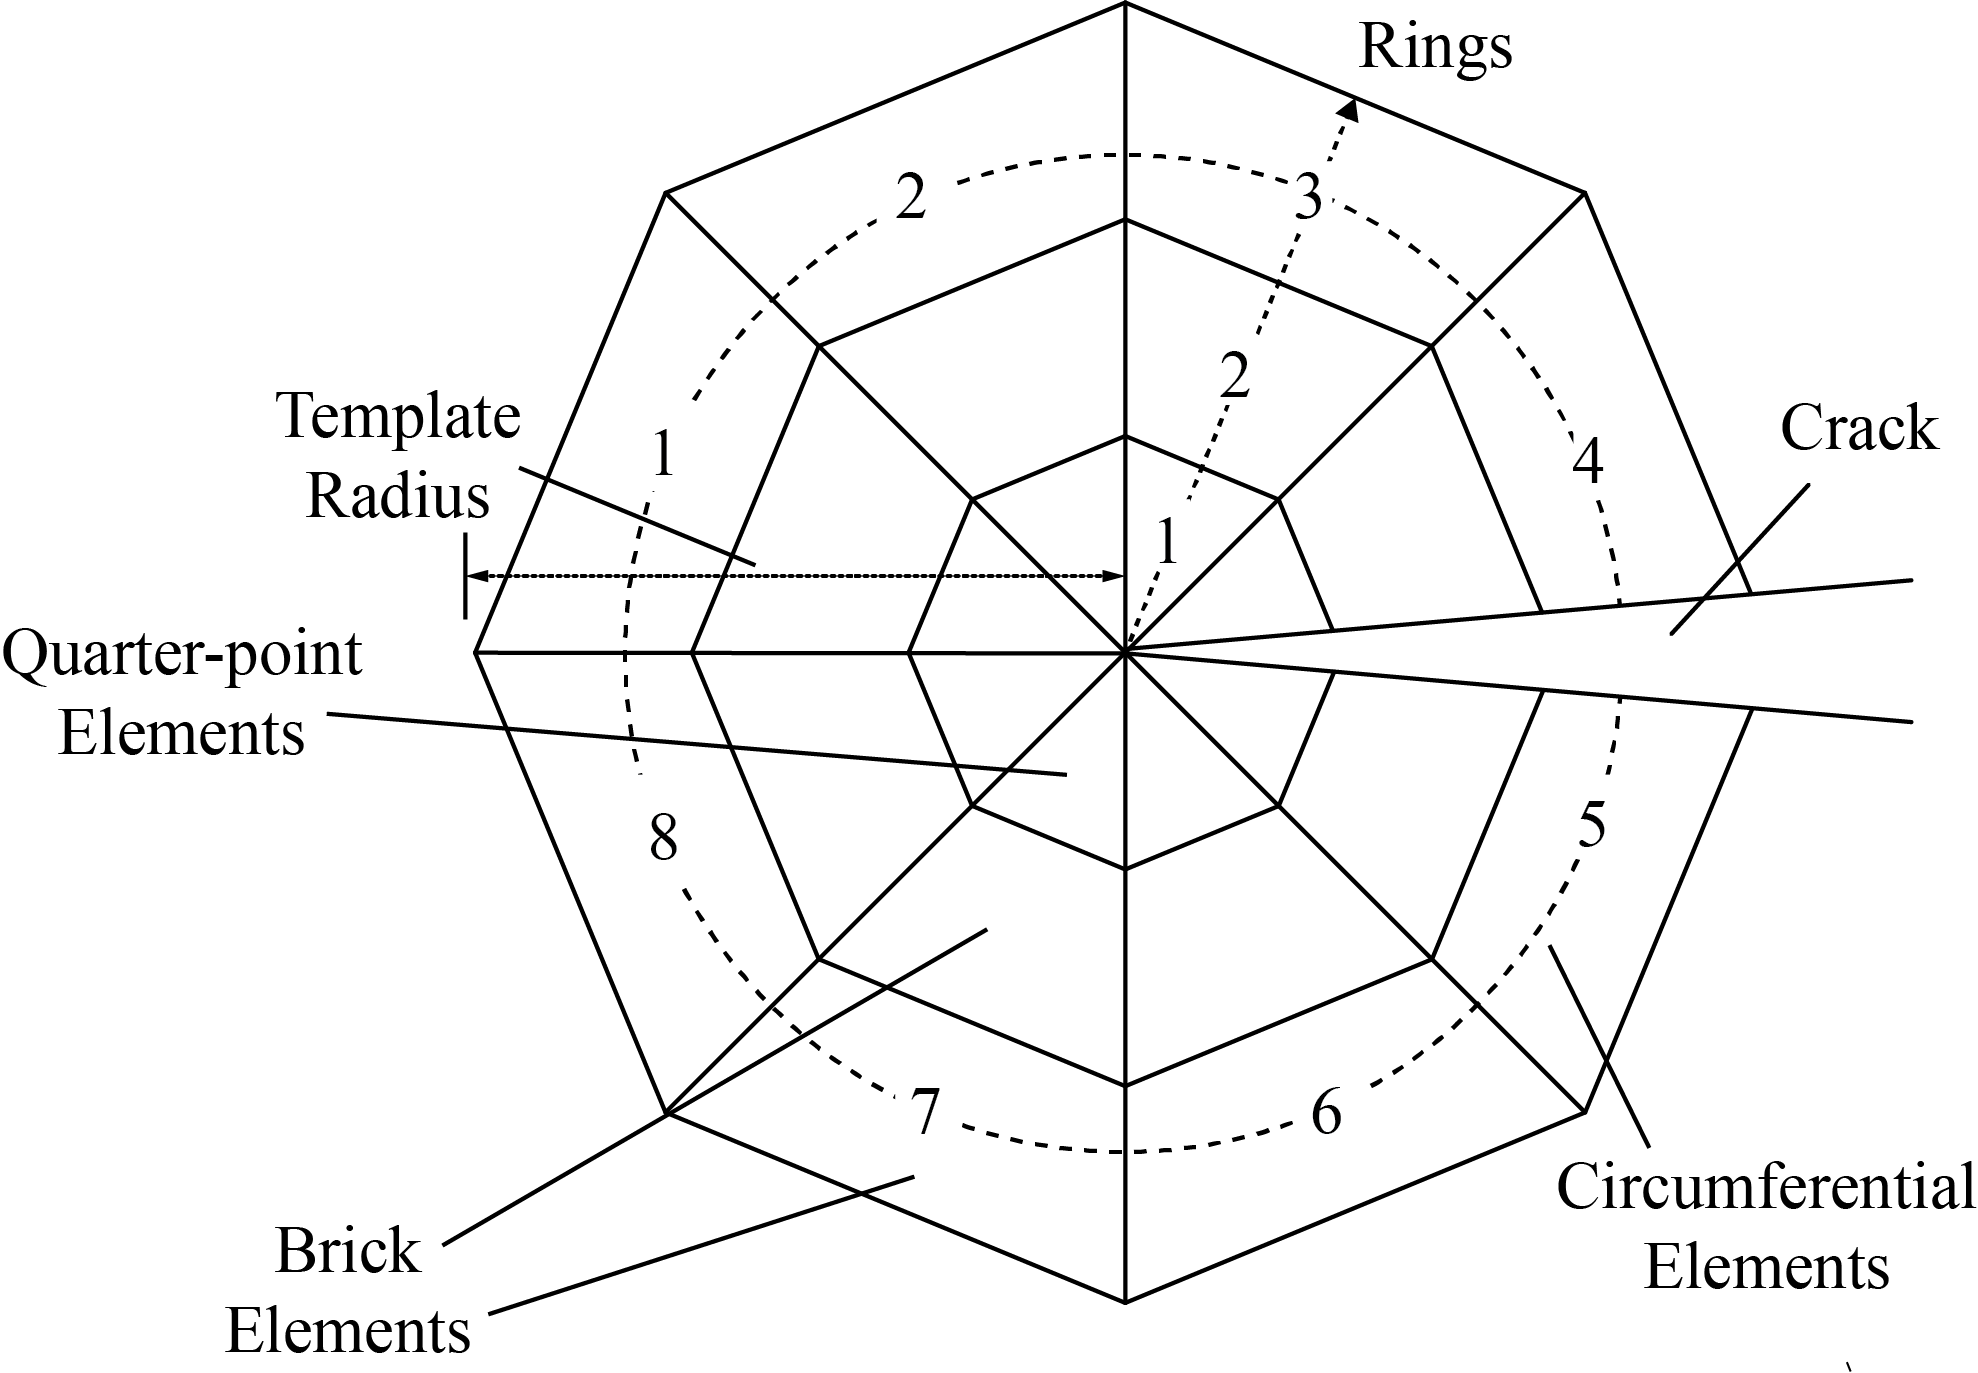
\includegraphics[width=0.8\textwidth]{geometry_figures/f3d_crack.png}
  \label{fig:f3d_mesh}
  \caption{FRANC3D crack mesh containing 8 circumferential elements and 3 rings. The template radius is the radius of an inscribed circle}
\end{figure}

Integral methods are geometrically more accurate than displacement methods, such as displacement correlation, for the computation of SIFs. The J-integral, developed by Rice \cite{Rice1968}, is a commonly used method for SIF calculation. However, it has a limitation, it cannot separate the SIFs into the three cracking modes, except for very simplified crack geometries, as noted by Banks-Sills et al. \cite{Banks-Sills2005}. Banks-Sills et al. developed the M-Integral formulation to overcome this limitation allowing for the calculation of accurarate SIFs for all three cracking modes \cite{Banks-Sills2005}

\begin{comment}

To address this limitation, the M-integral offers a solution by using a combination of two SIFs: one representing the true SIF and the other an arbitrary solution. By employing this approach, it becomes possible to extract each SIF corresponding to the three cracking modes, as explained by \cite{Banks-Sills2005}. The M-integral is defined as follows:

\begin{equation}\label{eqn:M-Integral}
    M^{(1, 2)} = \int_\Gamma \left(W^{(1,2)}n_1 - T^{(1)}_i \frac{\partial u^{(2)}_i}{\partial x_1} - T^{(2)}_i \frac{\partial u^{(1)}_i}{\partial x_1} \right) \, \text{d}s,
\end{equation}

Here, $T_i = \sigma_{ij} n_j$ represents the traction vector, $W = 1/2 \sigma_{ij} \epsilon_{ij}$ stands for the strain energy density, and the superscripts 1 and 2 correspond to the two superposed solutions.
\end{comment}

\subsection{Genetic Programming Based Symbolic Regression}
% look at previous papers to write this Karl, Donovan, Geoff plasticity paper
% https://arxiv.org/abs/2304.01117

Symbolic Regression (SR) is a machine learning technique aimed at discovering closed-form analytical expressions that model training data and known physics \cite{Karl,  Hongsup}. Presently, the most effective optimization approach for SR is genetic programming (GP) \cite{GPSR-comp}. The implementation of genetic programming based symbolic regression (GPSR) employed in this research is an open-source Python package, Bingo \cite{Randall2022}. Bingo enables learning real-valued mathematical expressions represented as acyclic graphs (Agraphs). The equation's complexity is determined by the number of nodes in the Agraph, Fig. \ref{fig:agraph} shows an Agraph for the equation $C_0 X_0 + C_1 X_1$, that has a complexity of 7 corresponding to the 7 nodes in the Agraph. The training begins with an initial assortment of randomly generated equations, varying in complexity. During each generation, equations undergo randomized evolutions, employing a combination of crossover and mutation. Crossover entails exchanging nodes from two Agraphs along with their associated branches and leaves, generating two evolved equations. Mutation introduces random changes to nodes in the Agraph as shown in Fig. \ref{fig:agraph_cross_mut} \cite{Schmidt2007}. After crossover and mutation has occurred the equations are ranked based on a defined fitness function e.g. MAE, RMSE, etc. The most fit equations are then used in the next generation where the cycle continues until a fitness threshold or maximum number of generations has been satisfied. 

\begin{figure}
    \centering
    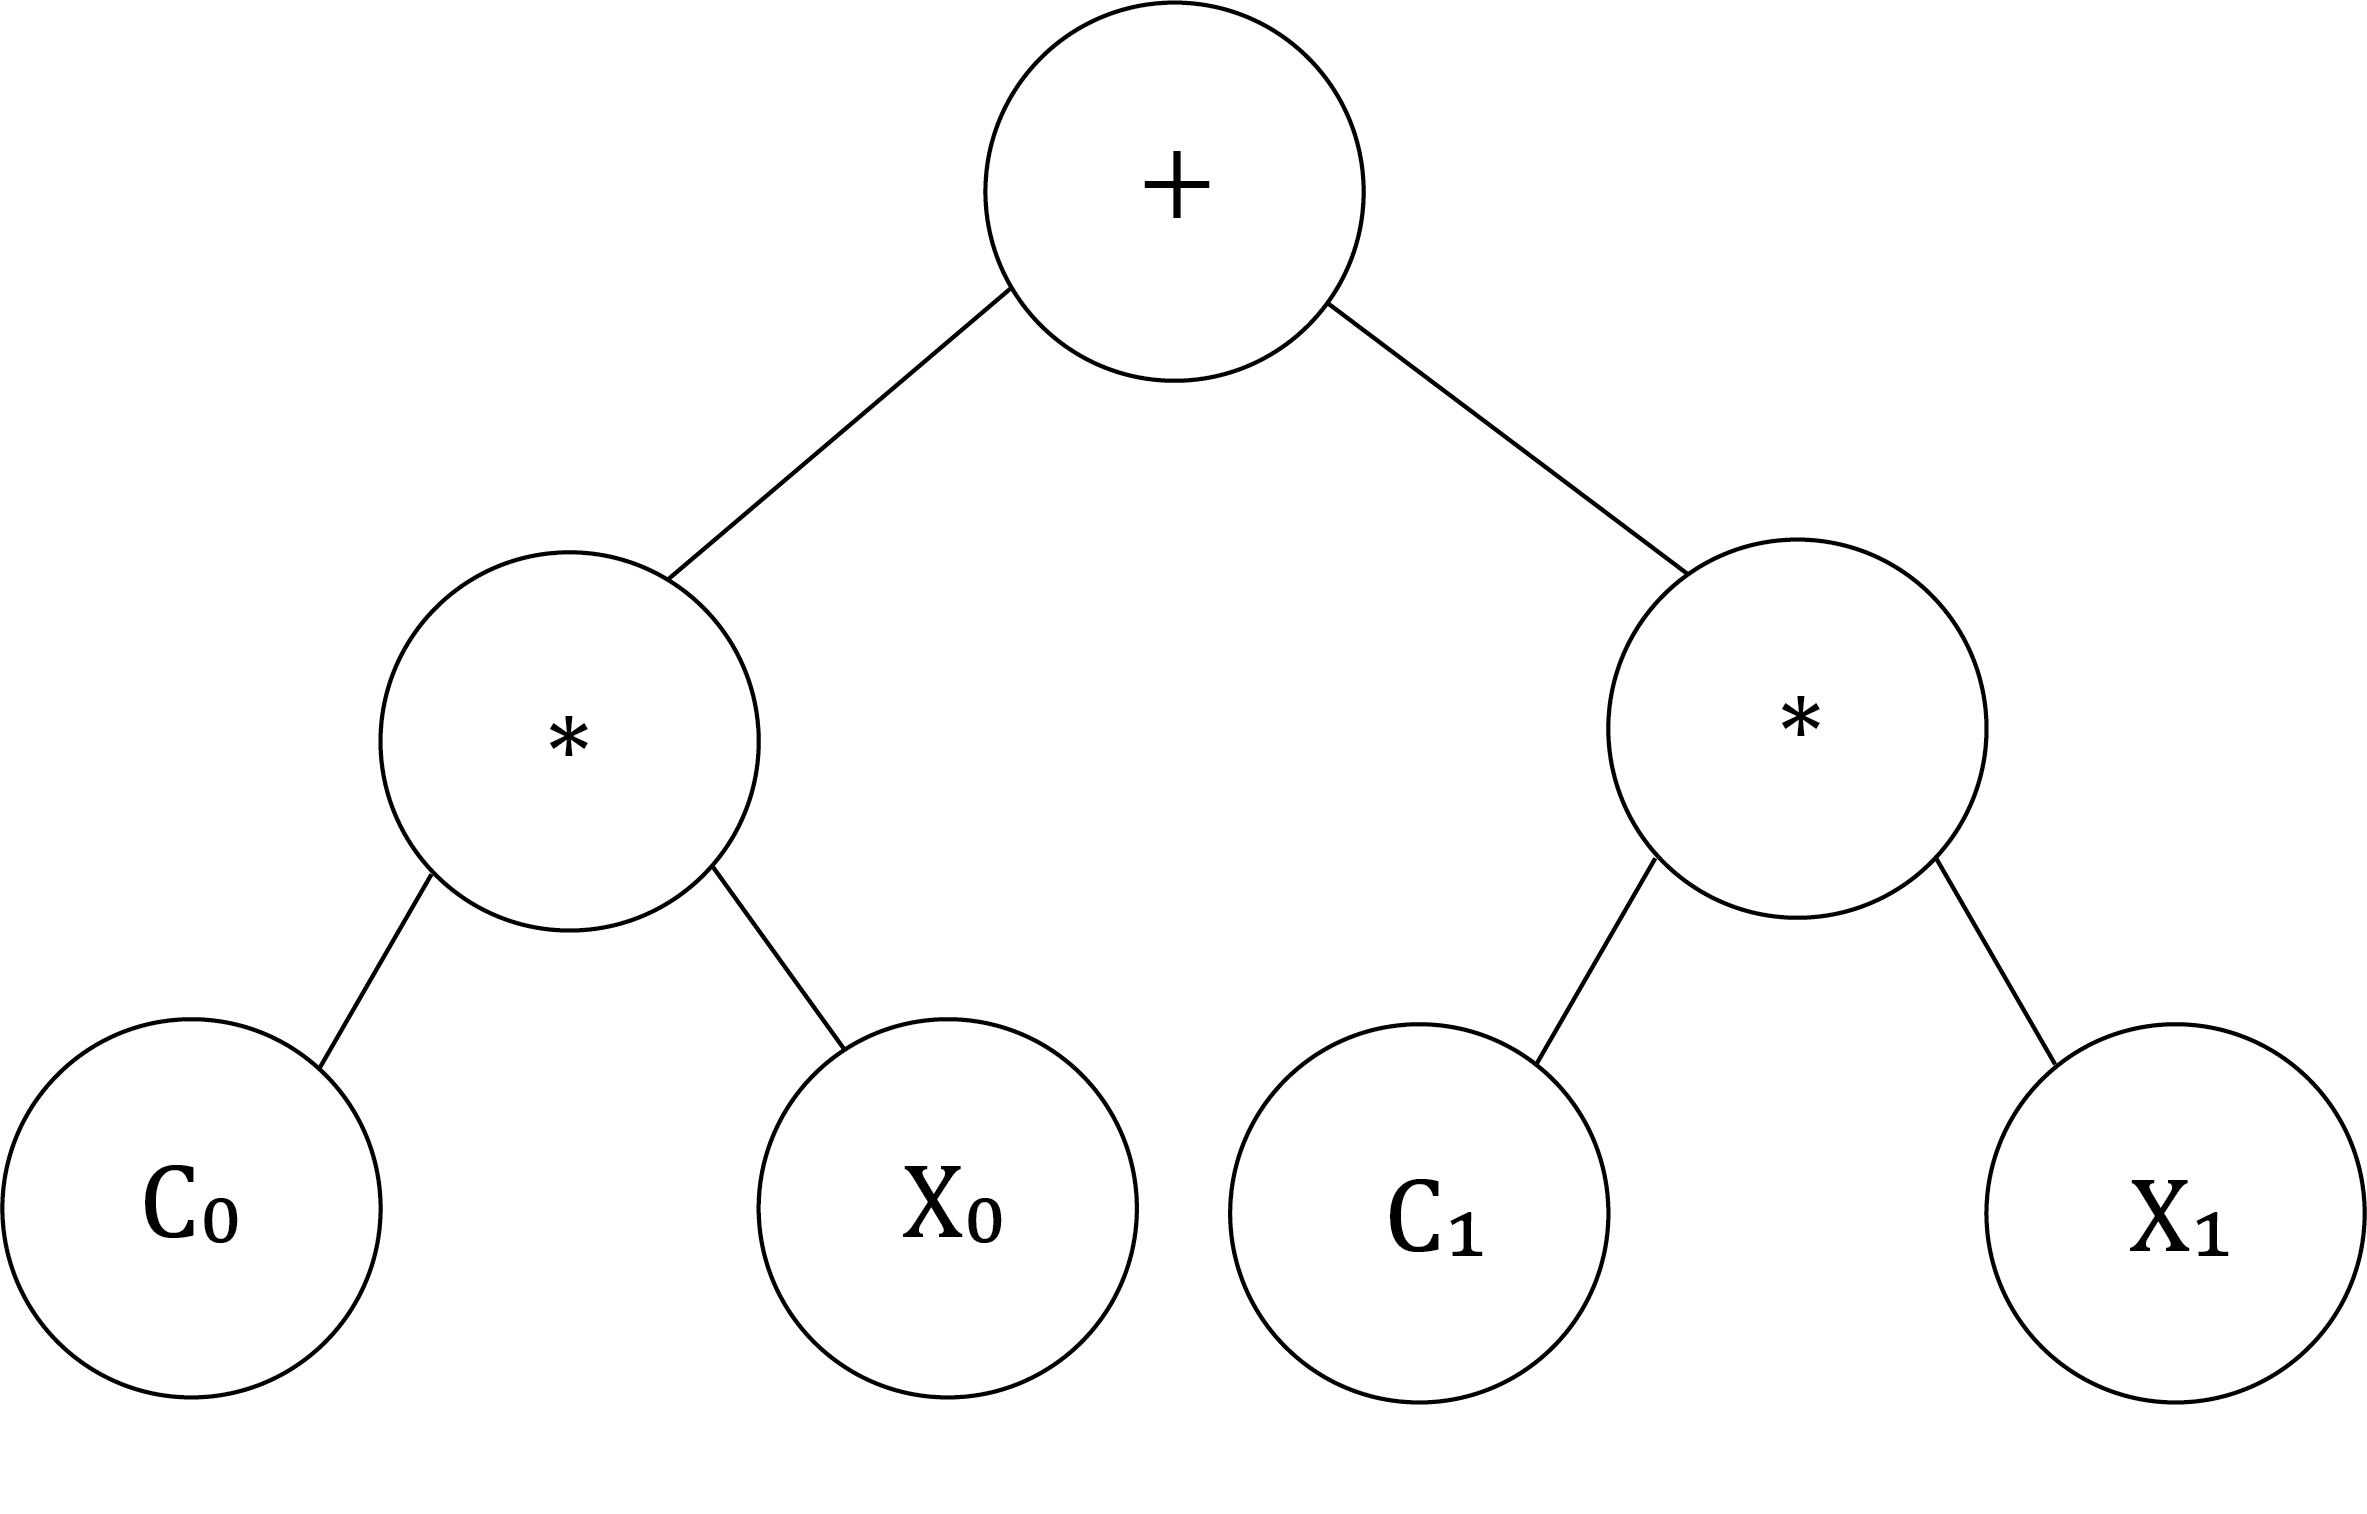
\includegraphics[width=0.6\textwidth]{geometry_figures/agraph.png}
    \label{fig:agraph}
    \caption{Example Agraph for for equation; $C_0 X_0 + C_1 X_1$, where the complexity is the sum of the nodes in this case 7.} 
\end{figure}


\begin{figure}
    \centering

    \begin{minipage}{\textwidth}
        \centering
        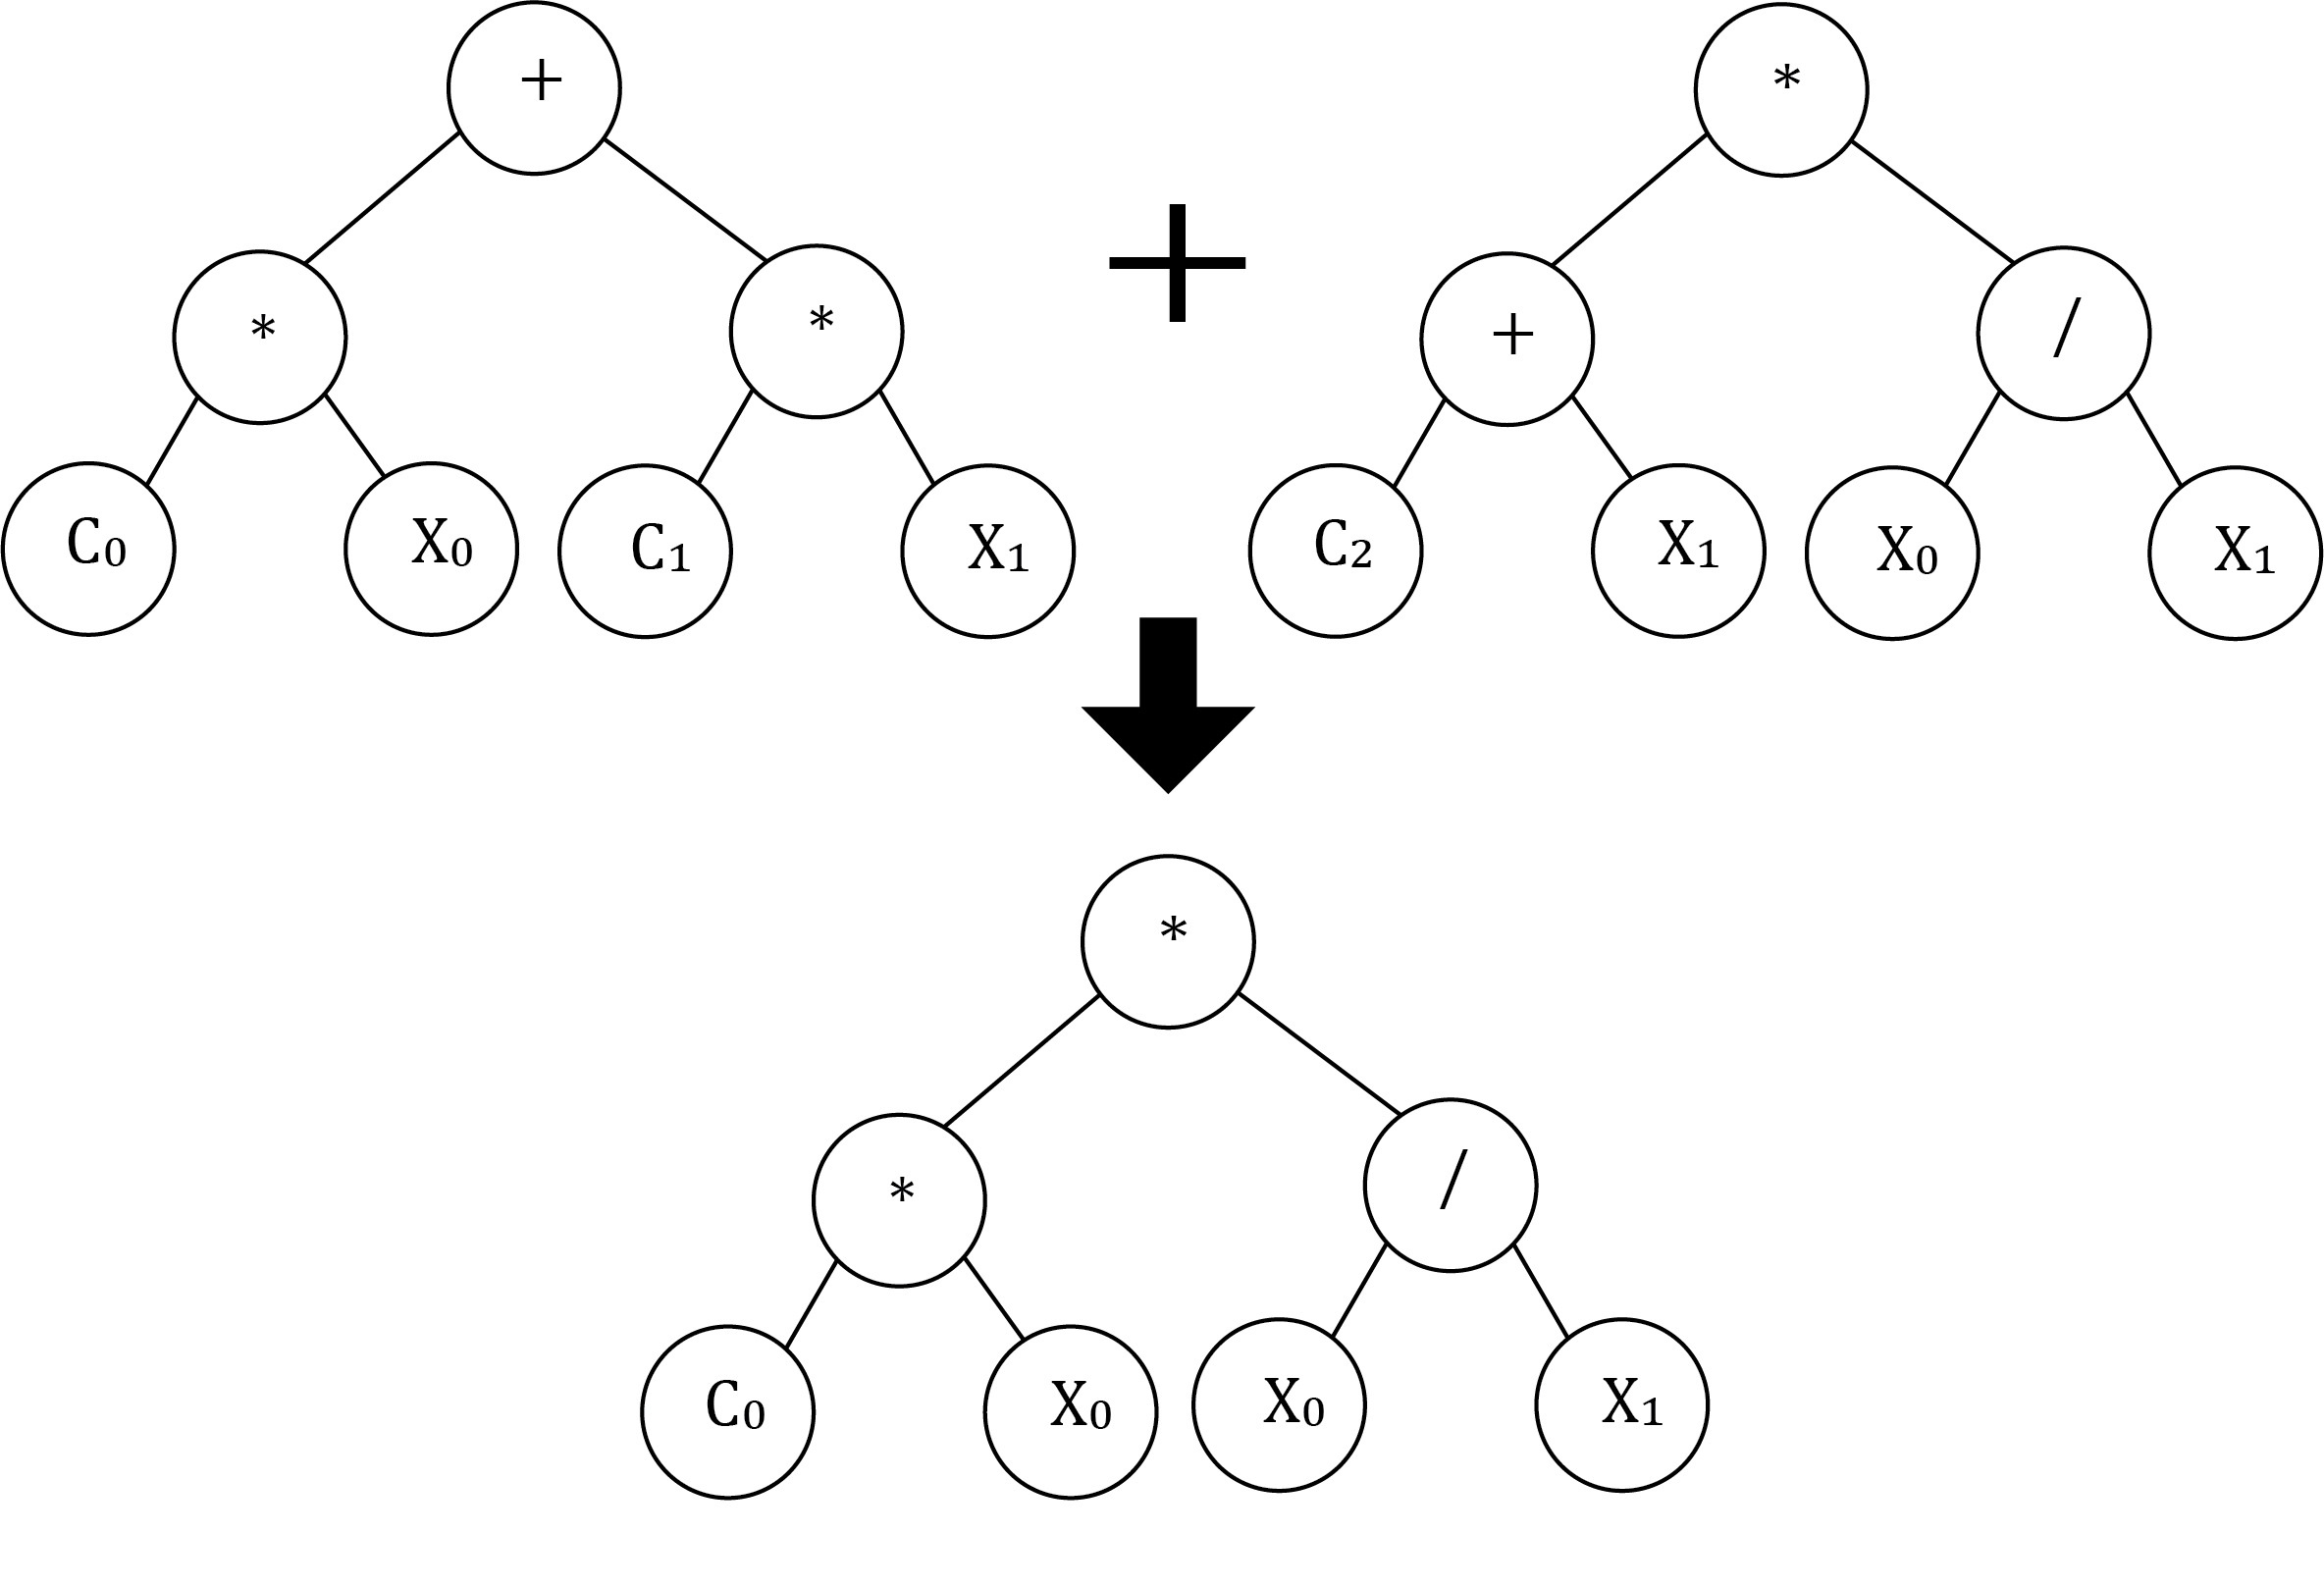
\includegraphics[width=0.8\linewidth]{geometry_figures/agraph-crossover.png}
        \caption*{(a)}
    \end{minipage}
    
    \begin{minipage}{\textwidth}
        \centering
        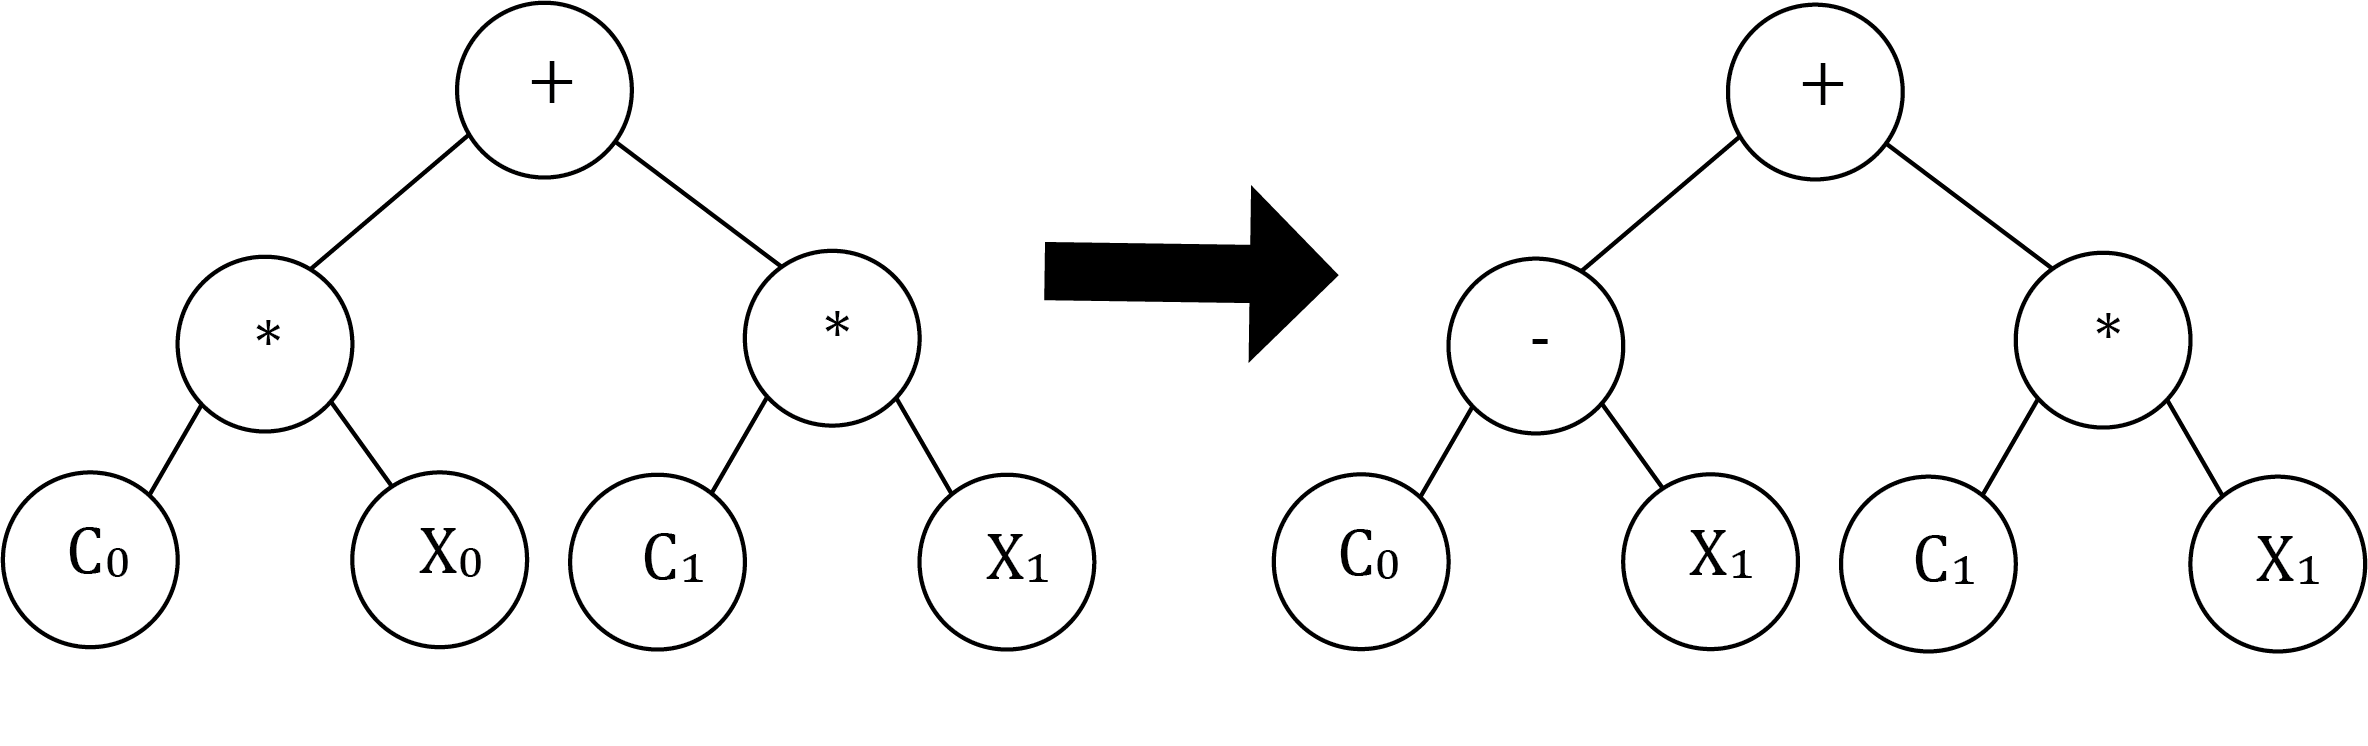
\includegraphics[width=0.8\linewidth]{geometry_figures/agraph-mutation.png}
        \caption*{(b)}
    \end{minipage}
    
    \caption{(a) crossover, where two parent graphs combine features to create a child graph. (b) where part of a graph is randomly changed creating a new graph.}
    \label{fig:agraph_cross_mut}
\end{figure}




The most fit equations, at various complexity values, from the final population are taken and presented as a Pareto front Fig. \ref{fig:perato-front}. Equations with high complexity have better fitness values; however, they often have reduced interpretabiliy from the engineer's perspective. Equations with low complexity tend to be easily interpreteble at the expense of decreased fitness. Lacking additional criteria, a user must decide what equation is the best for the application. Typically, there is a point at which increasing the complexity yields little gain on fitness Fig. \ref{fig:perato-front}, which serves as a balance between accuracy and complexity. ***anotate plot****

\begin{figure}
    \centering
    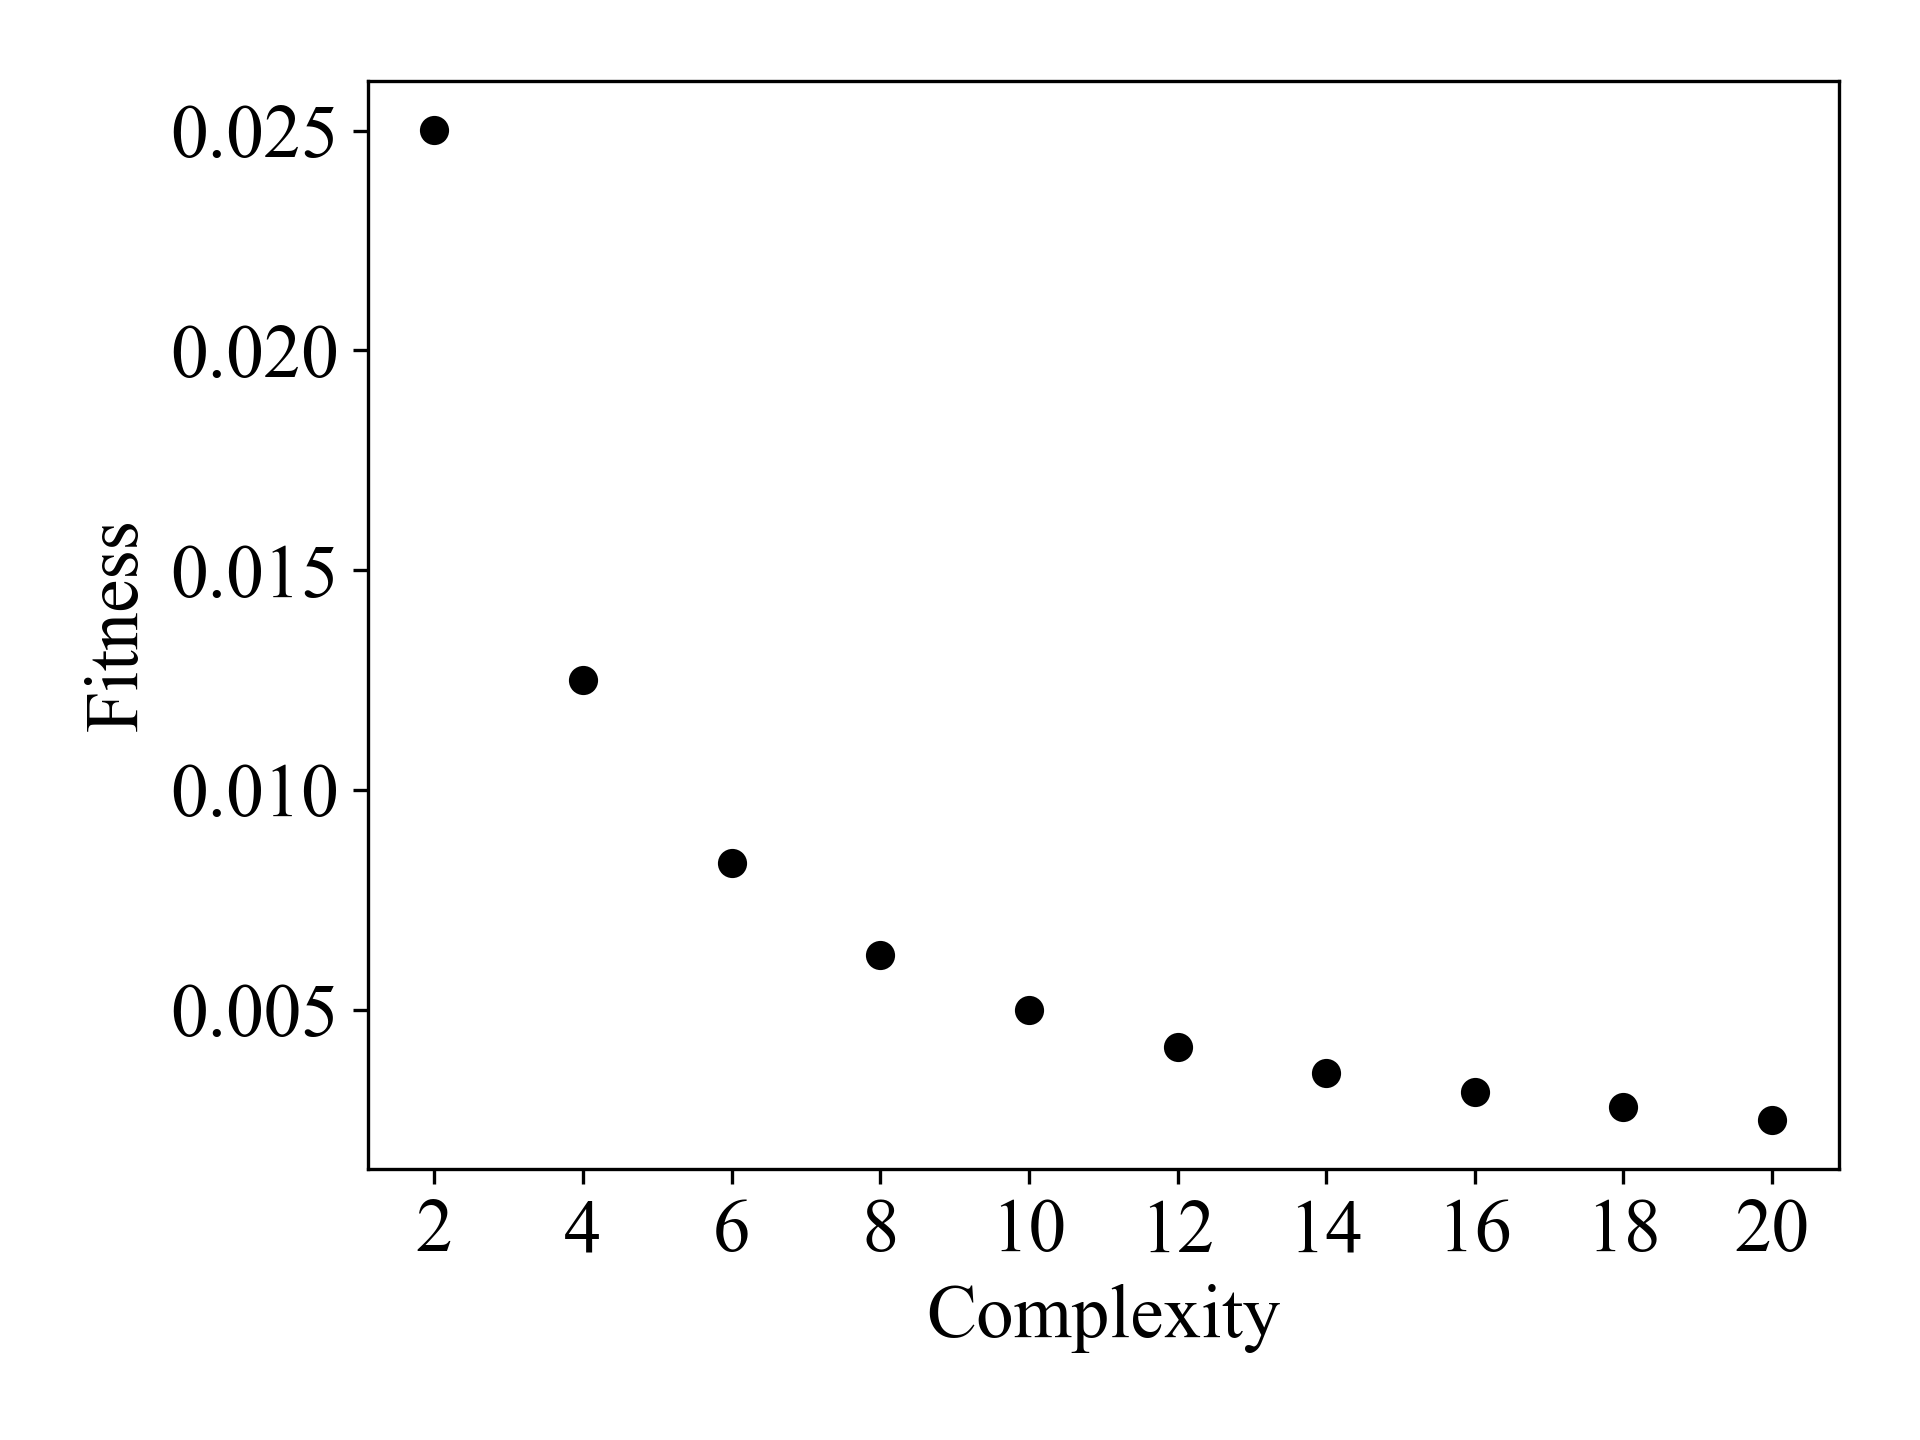
\includegraphics[width=0.6\textwidth]{Figures/dummy_pareto_front.png}
    \label{fig:perato-front}
    \caption{Example Pareto front where the horizontal axis is the model complexity and the vertical axis is the model fitness. Each point on the graph represents a different model in the population.} 
\end{figure}




 